\documentclass[11pt]{article}
\usepackage[usenames]{color} %used for font color
\usepackage{amssymb} %maths
\usepackage{amsmath} %maths

\usepackage[no-math]{fontspec}
\usepackage{unicode-math}
\usepackage{libertinus}

\usepackage{pgf,xcolor}
\definecolor{itwm_blue_04}{HTML}{005A94}
\definecolor{itwm_red}{HTML}{C00000}

\usepackage{tikz}
\usetikzlibrary{shapes.misc, shadows, decorations, arrows}
\usetikzlibrary{backgrounds}
\usetikzlibrary{calc}
\usepackage{pgfplots}
\pgfplotsset{compat=newest}
\usepgfplotslibrary{fillbetween}
\usepackage{tikzpagenodes}
\usetikzlibrary{decorations.markings}\begin{document}
\begin{align*}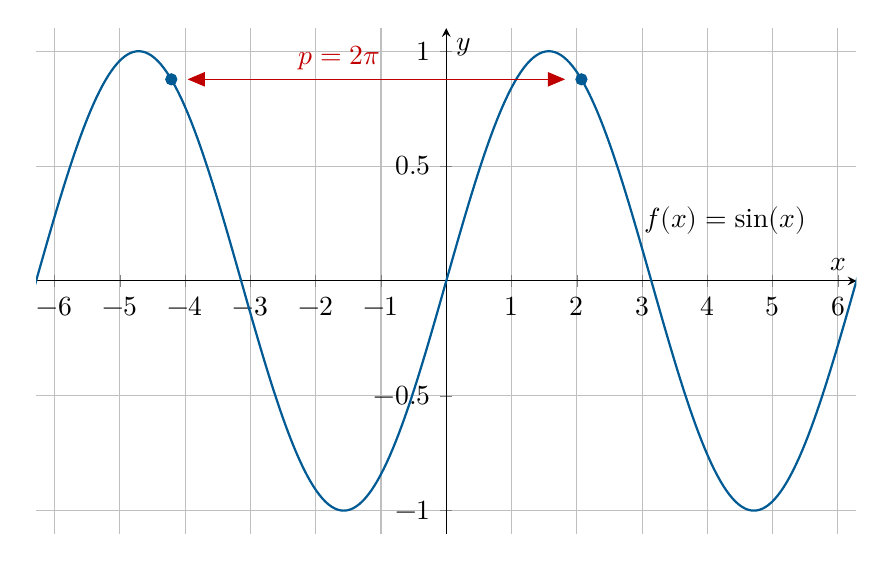
\begin{tikzpicture}[>=triangle 45,]
\begin{axis}[
    domain=-7:7,
    axis lines = center,
    xlabel = {$x$},
    ylabel = {$y$},
    height=8cm, width=12cm, 
    xmin=-2*pi, xmax=2*pi, ymin=-1.1, ymax=1.1, 
    xtick={-6, -5,...,6},
    ytick={-1,-0.5,...,1},
    grid = both
]
\path [name path=xaxis]
      (\pgfkeysvalueof{/pgfplots/xmin},0) --
      (\pgfkeysvalueof{/pgfplots/xmax},0);
\addplot[draw=itwm_blue_04, samples=300, thick, name path=f]{sin(deg(x))} node [pos=0.7, right] {$f(x)=\sin(x)$};
\addplot [<->, color=itwm_red] coordinates {(-4.2123 + 0.25,0.877583) (2.0708 - 0.25, 0.877583)} node [pos=0.4, above] {$p=2\pi$};
\addplot [mark=*, color=itwm_blue_04] coordinates {(-4.2123,0.877583)};
\addplot [mark=*, color=itwm_blue_04] coordinates {(2.0708, 0.877583)};
\end{axis}
\end{tikzpicture}\end{align*}
\end{document}